\documentclass[12pt, a4paper]{article}
\usepackage[utf8]{inputenc}
\usepackage[english]{babel}
\usepackage{amsmath}
\usepackage{amsfonts}
\usepackage{amssymb}
\usepackage{siunitx}
\usepackage{longtable}
\usepackage[margin=1in]{geometry}
\usepackage{graphicx}
\usepackage{float}

\begin{document}

\begin{center}
	\Large \textbf{1: VISCOSITY COEFFICIENT OF GLYCERIN}
	\vspace{0.5cm}
	    
	\normalsize Marmara University - Department of Physics \\
	Physics 3 Laboratory \\
	Experiment Report
	\vspace{0.5cm}
\end{center}

\section{Objective}
The purpose of this experiment is to measure the viscosity coefficient ($\eta$) of a viscous liquid, glycerin, using Stokes' Law.

\section{Theoretical Background}
Stokes' Law states that a friction force acts on a globe moving in a viscous liquid, given by $F_v = 6\pi\eta vr$, where $\eta$ is the viscosity coefficient, $v$ is the velocity of the sphere, and $r$ is the radius. Initially, with no speed, only gravity ($F_g = mg = \frac{4}{3}\pi r^3 \rho_2 g$) and ascending force ($F_a = \rho_1 V g = \frac{4}{3}\pi r^3 \rho_1 g$) act, where $\rho_1$ and $\rho_2$ are liquid and globe densities, and $V$ is the volume of the submerged sphere. The initial acceleration is $a = \frac{\rho_2 - \rho_1}{\rho_2}g$. As speed increases, friction grows, and at terminal speed, there is no acceleration since $F_g - F_a = F_v$, yielding $\eta = \frac{2}{9} \frac{(\rho_2 - \rho_1)g r^2}{v}$.

\section{Apparatus and Method}
The experiment utilized glycerin, a graduated cylinder, two steel balls with diameters of 0.47 cm and 0.30 cm, a stopwatch, a caliper for diameter measurement, a ruler to measure the distance between measurement points, and a magnet for controlled ball release. The experimental procedure involved filling the graduated cylinder with glycerin, measuring ball diameters with a caliper, marking levels A and B at the 200 ml and 100 ml marks respectively (distance $L = \SI{7.4}{\centi\metre}$ measured with ruler), using the magnet to release each ball from the top of the cylinder, recording the falling time between the 200-100 ml marks, then using the magnet to lift each ball back to the top and repeating this process three times for each ball to calculate the average falling time.

\section{Measurements and Data}
Constants:
\begin{itemize}
	\item Mass density of steel ball: $\rho_2 = \SI{7870}{\kilo\gram\per\metre\cubed}$
	\item Mass density of glycerin: $\rho_1 = \SI{900}{\kilo\gram\per\metre\cubed}$
	\item Gravitational acceleration: $g = \SI{9.80}{\metre\per\second\squared}$
	\item Length of A-B: $L = \SI{7.4}{\centi\meter}$
\end{itemize}

\begin{small}
	\begin{longtable}{|c|c|c|c|c|c|c|c|c|c|}
		\caption{Glycerin Viscosity Measurement and Calculation} \label{tab:olcum} \\
		\hline
		\textbf{Ball} & \textbf{d} (\si{cm}) & \textbf{r} (\si{cm}) & \textbf{$r^2$} (\si{m^2}) & \multicolumn{3}{c|}{\textbf{Time, $t$} (\si{s})} & \textbf{$t_{avg}$} (\si{s}) & \textbf{$V$} (\si{m/s}) & \textbf{$\eta$} (\si{Pa.s}) \\
		\cline{5-7}
		  &        &         &                       & \textbf{$t_1$} & \textbf{$t_2$} & \textbf{$t_3$} &       &        &        \\
		\hline
		1 & 0.47 & 0.235 & $5.52 \times 10^{-6}$ & 0.61           & 0.68           & 0.49           & 0.593 & 0.1248 & 0.6717 \\
		2 & 0.30 & 0.150 & $2.25 \times 10^{-6}$ & 1.73           & 1.72           & 1.64           & 1.70  & 0.0435 & 0.7851 \\
		\hline
		\multicolumn{9}{|r|}{\textbf{Mean $\eta_{avg}$}} & 0.7284 \\
		\hline
	\end{longtable}
\end{small}

\section{Calculations and Graphs}
The viscosity coefficients are calculated using the terminal velocity ($V = L / t_{\text{avg}}$) and the formula $\eta = \frac{2}{9} \frac{(\rho_2 - \rho_1) g r^2}{V}$.

For ball 1: $\eta_1 = \SI{0.6717}{\pascal\second}$  
For ball 2: $\eta_2 = \SI{0.7851}{\pascal\second}$  

\[ \eta_{\text{avg}} = \frac{0.6717 + 0.7851}{2} = \SI{0.7284}{\pascal\second} \]

The slope ($m$) of the $V$ vs. $r^2$ graph is calculated using the two data points:
\[ m = \frac{0.1248 - 0.0435}{(5.5225 \times 10^{-6}) - (2.25 \times 10^{-6})} = \frac{0.0813}{3.2725 \times 10^{-6}} \approx \SI{24844}{\per\metre\per\second} \]

The viscosity coefficient based on the slope:
\[ \eta_{\text{graph}} = \frac{2 g (\rho_2 - \rho_1)}{9 m} = \frac{2 \times 9.80 \times (7870 - 900)}{9 \times 24844} \approx \SI{0.611}{\pascal\second} \]

\subsection{Graph}
\begin{figure}[H]
	\centering
	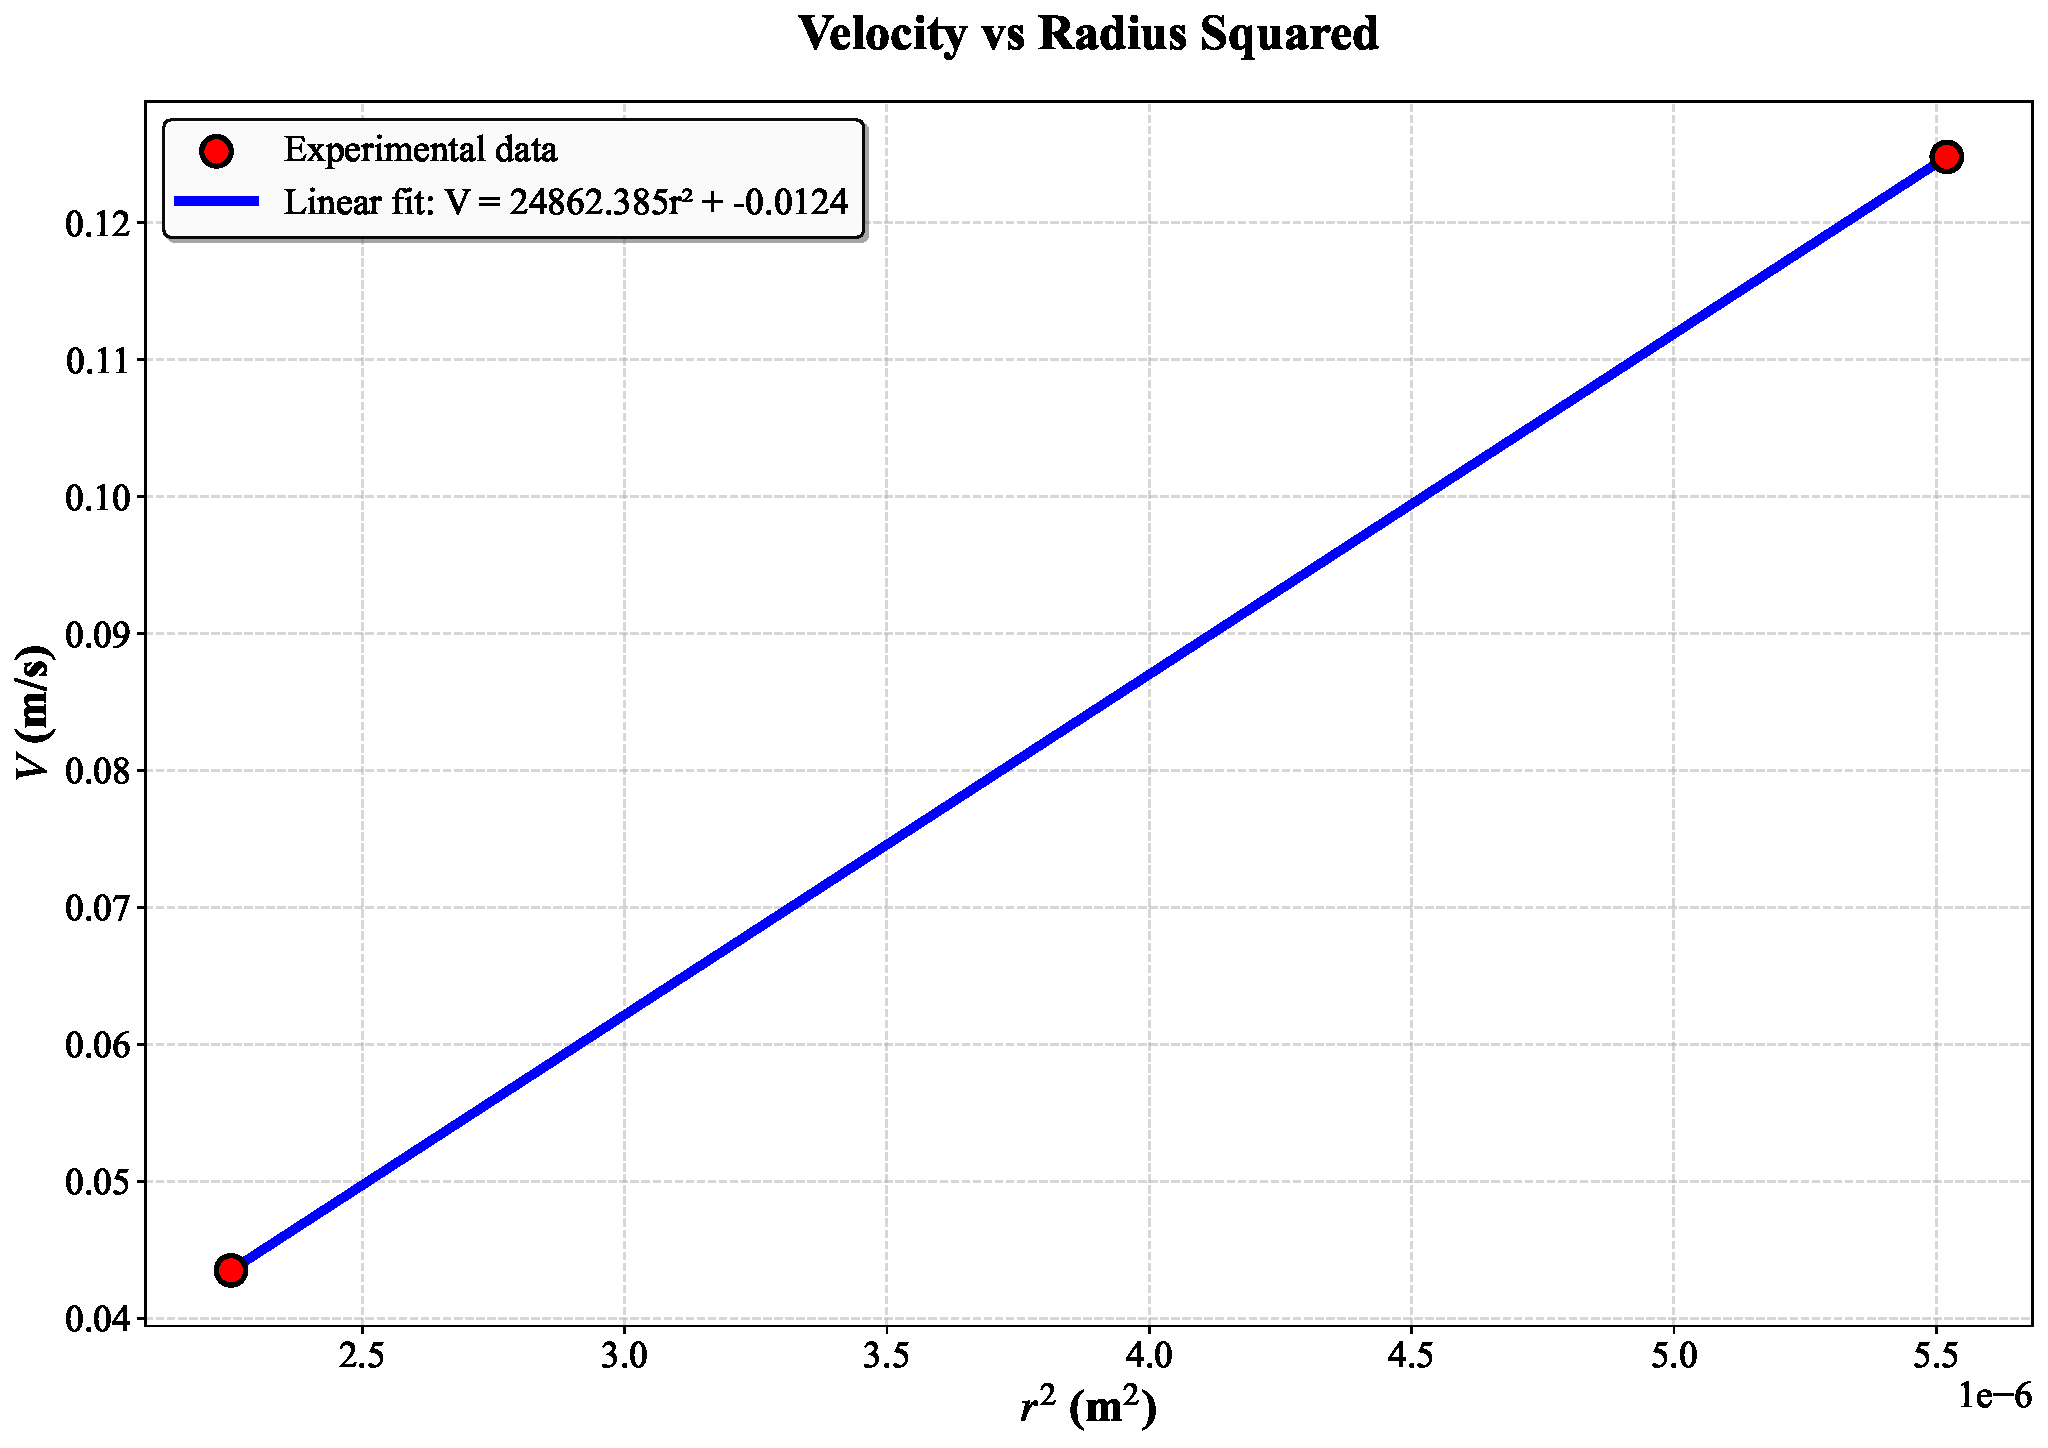
\includegraphics[width=0.8\textwidth]{velocity_vs_radius_squared.pdf}
	\caption{$V$ vs. $r^2$ graph}
\end{figure}

\section{Results and Discussion}
The viscosity coefficient of glycerin was determined through the application of Stokes' Law using falling metal spheres. Two calculation methods yielded viscosity values of $\eta_{\text{avg}} = \SI{0.7284}{\pascal\second}$ (direct calculation) and $\eta_{\text{graph}} = \SI{0.611}{\pascal\second}$ (graphical analysis). The experimental results validated the expected theoretical behavior, demonstrating a distinct relationship between sphere radius and terminal velocity. The measurements were conducted in the lower section of the cylinder to ensure accurate terminal velocity data collection.

The main reason for differences between our measured values and theoretical values was that the glycerin was not pure. We could not guarantee the purity of the glycerin, which affected our viscosity measurements. The glycerin may have become impure because it was left open for a long time and absorbed moisture from the humid air in the room. The differences between our experimental results and literature values for pure glycerin are mainly due to this impurity problem and the small number of data points we collected.

Sources of error:
\begin{enumerate}
	\item Glycerin impurity/contamination from humid storage, leading to water absorption and reduced viscosity/density (major source; explains discrepancy with literature).
	\item Limited data (only two balls), reducing statistical reliability and robustness of the slope.
\end{enumerate}

\newpage

\textbf{Student Information}

Name Surname: Hakkı Erdem Günal

Student ID: 173223024

Course: Physics 3 Laboratory

Experiment No / Title: 2 / Viscosity Coefficient of Glycerin

Experiment Date: September 29, 2025

Submission Date: October 5, 2025

\end{document}

